\chapter{Лабораторная работа №7\\\eng{FLASH} память} 

\section{Виды энергонезависимой памяти}

\par{Ни один из блоков цифровых устройств, которые мы рассмотрели ранее не способен хранить информацию при отсутствии питания.}

\par{Чтобы решить эту проблему, на заре вычислительной техники, данные в цифровое устройство после подачи питания загружали с таких носителей, как перфокарты и, позже, магнитные ленты. Ещё позже для этих целей были разработаны накопители на гибких магнитных дисках --- дискетах и жёстких магнитных дисках --- \qeng{HDD}. На данный момент для хранения данных при отсутствии питания наиболее широко применяется \eng{FLASH}-память.}

\par{Энергонезависимые накопители информации обладают как преимуществами, так и недостатками по сравнению с энергозависимой \eng{RAM}-памятью.} 

\par{Как правило, энергонезависимая память существенно уступает по скорости работы \eng{RAM}-памяти. Это ограничение удалось преодолеть только недавно: в 2016 году была представлена постоянная память, где информация хранится в виде спина электрона. Такая память по скорости работы не уступает современной \eng{RAM}-памяти, такой как \eng{DDR5}. Но подобная память ещё долгое время будет  недоступна для рядового пользователя из-за высокой стоимости.}

\section{Принципы работы \eng{FLASH}-памяти}

\par{В качестве элемента хранения информации \eng{FLASH}-память использует транзистор с плавающим затвором. Состояние затвора определяет бит хранимой информации.}
\par{На Рис.\ref{fig:floating_gate_transistor} схематично изображена структура такого транзистора.}

\begin{figure}[H]
\centering
% \def\svgwidth{\columnwidth}
% \includesvg{floating_gate_transistor}
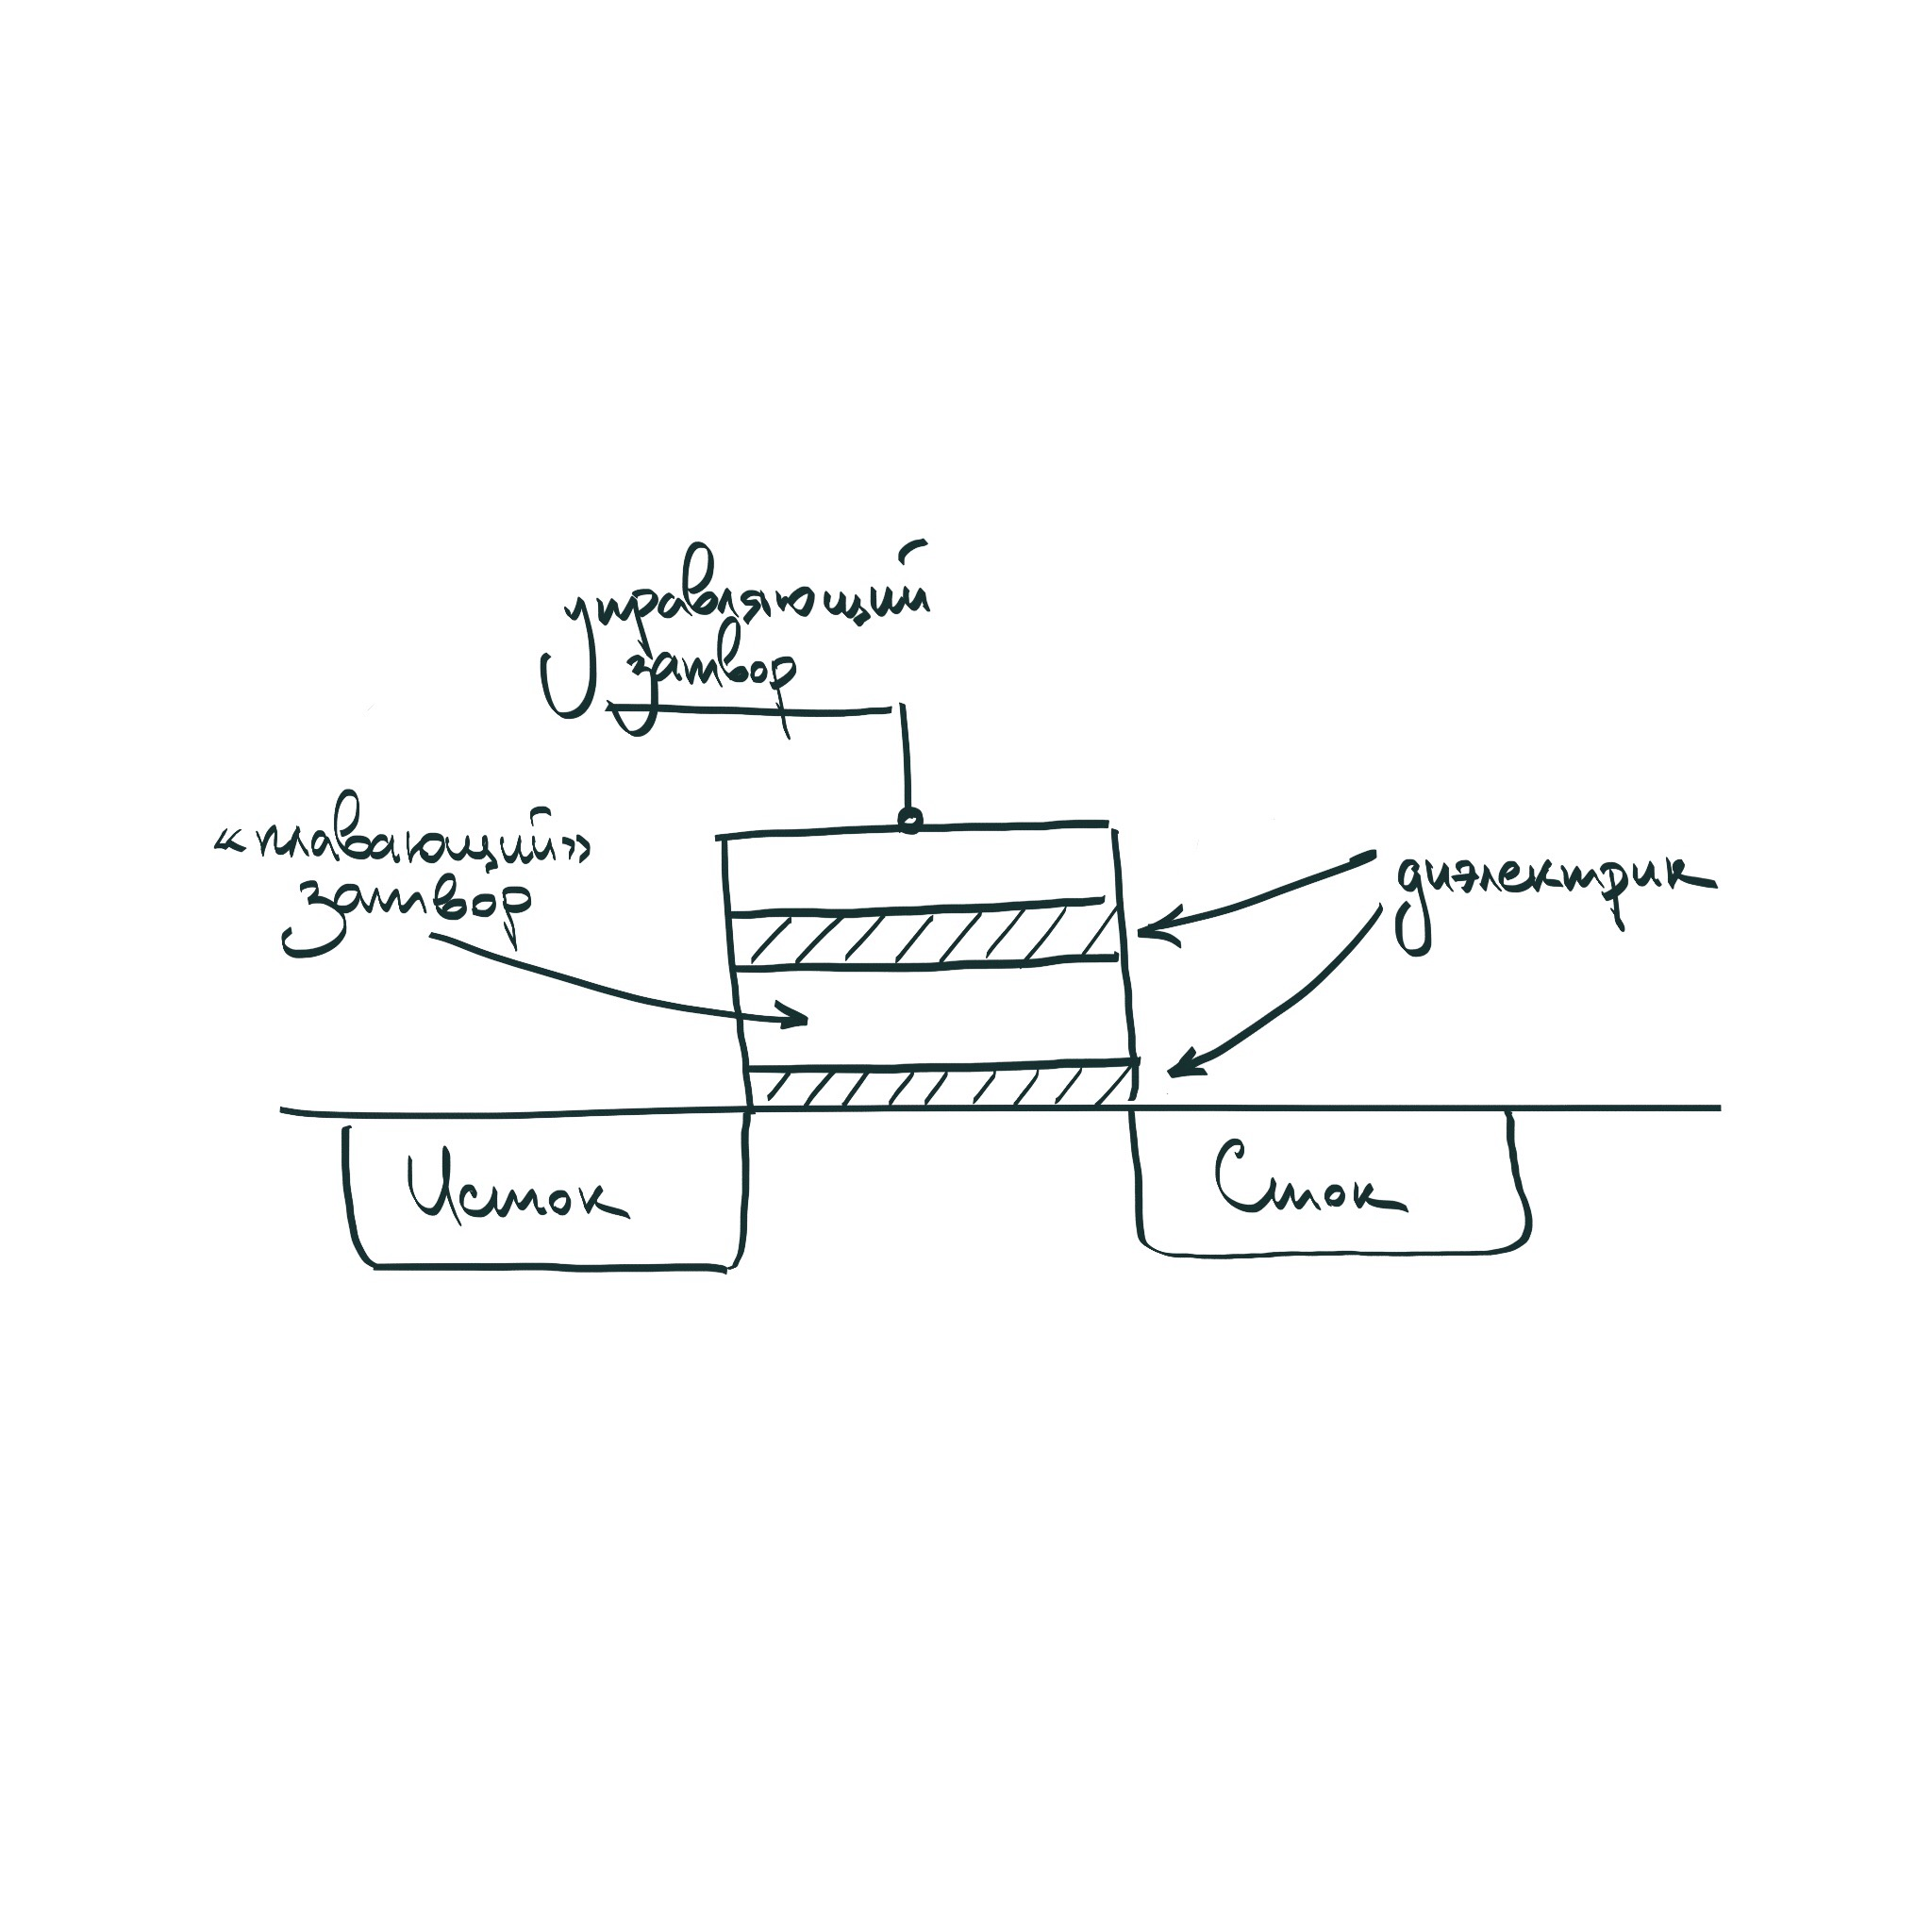
\includegraphics[width=0.8\textwidth]{./images/lab_6/floating_gate_transistor}
\caption{Транзистор с плавающим затвором}
\label{fig:floating_gate_transistor}
\end{figure}

\par{Как вы видите, он содержит два затвора: управляющий и плавающий. Плавающий затвор --- это полупроводник, который полностью окружён диэлектриком. При этом плавающий затвор способен накапливать электроны.}
\par{От величины накопленного заряда меняется \quotes{лёгкость}, с которой транзистор открывается --- т.е. величина напряжения \quotes{управляющий затвор---исток}, при котором через транзистор начнёт течь ток.}
\par{Чем больше электронов находятся в плавающем затворе, тем \quotes{легче} открывается транзистор --- ток начинает протекать через него при меньшем напряжении \quotes{управляющий затвор---исток}.}

\par{На Рисунке \ref{fig:floating_gate_read} изображены вольт-амперные характеристики транзистора с плавающем затвором в двух разных состояниях: когда в плавающем затворе накоплен отрицательный заряд и когда плавающий затвор не имеет заряда.}
\par{Для хранения информации используют следующий принцип: чтобы считать информацию, на управляющий затвор подаётся напряжение чтения --- среднее между самым сильным и самым слабым напряжением, способным открыть затвор. Если транзистор открывается, значит в плавающем затворе были электроны и мы считаем, что в нём записано значение \quotes{0}, если не открывается, значит электронов в плавающем затворе нет и записано значение \quotes{1}.}

\begin{figure}[H]
\centering
% \def\svgwidth{\columnwidth}
% \includesvg{floating_gate_read}
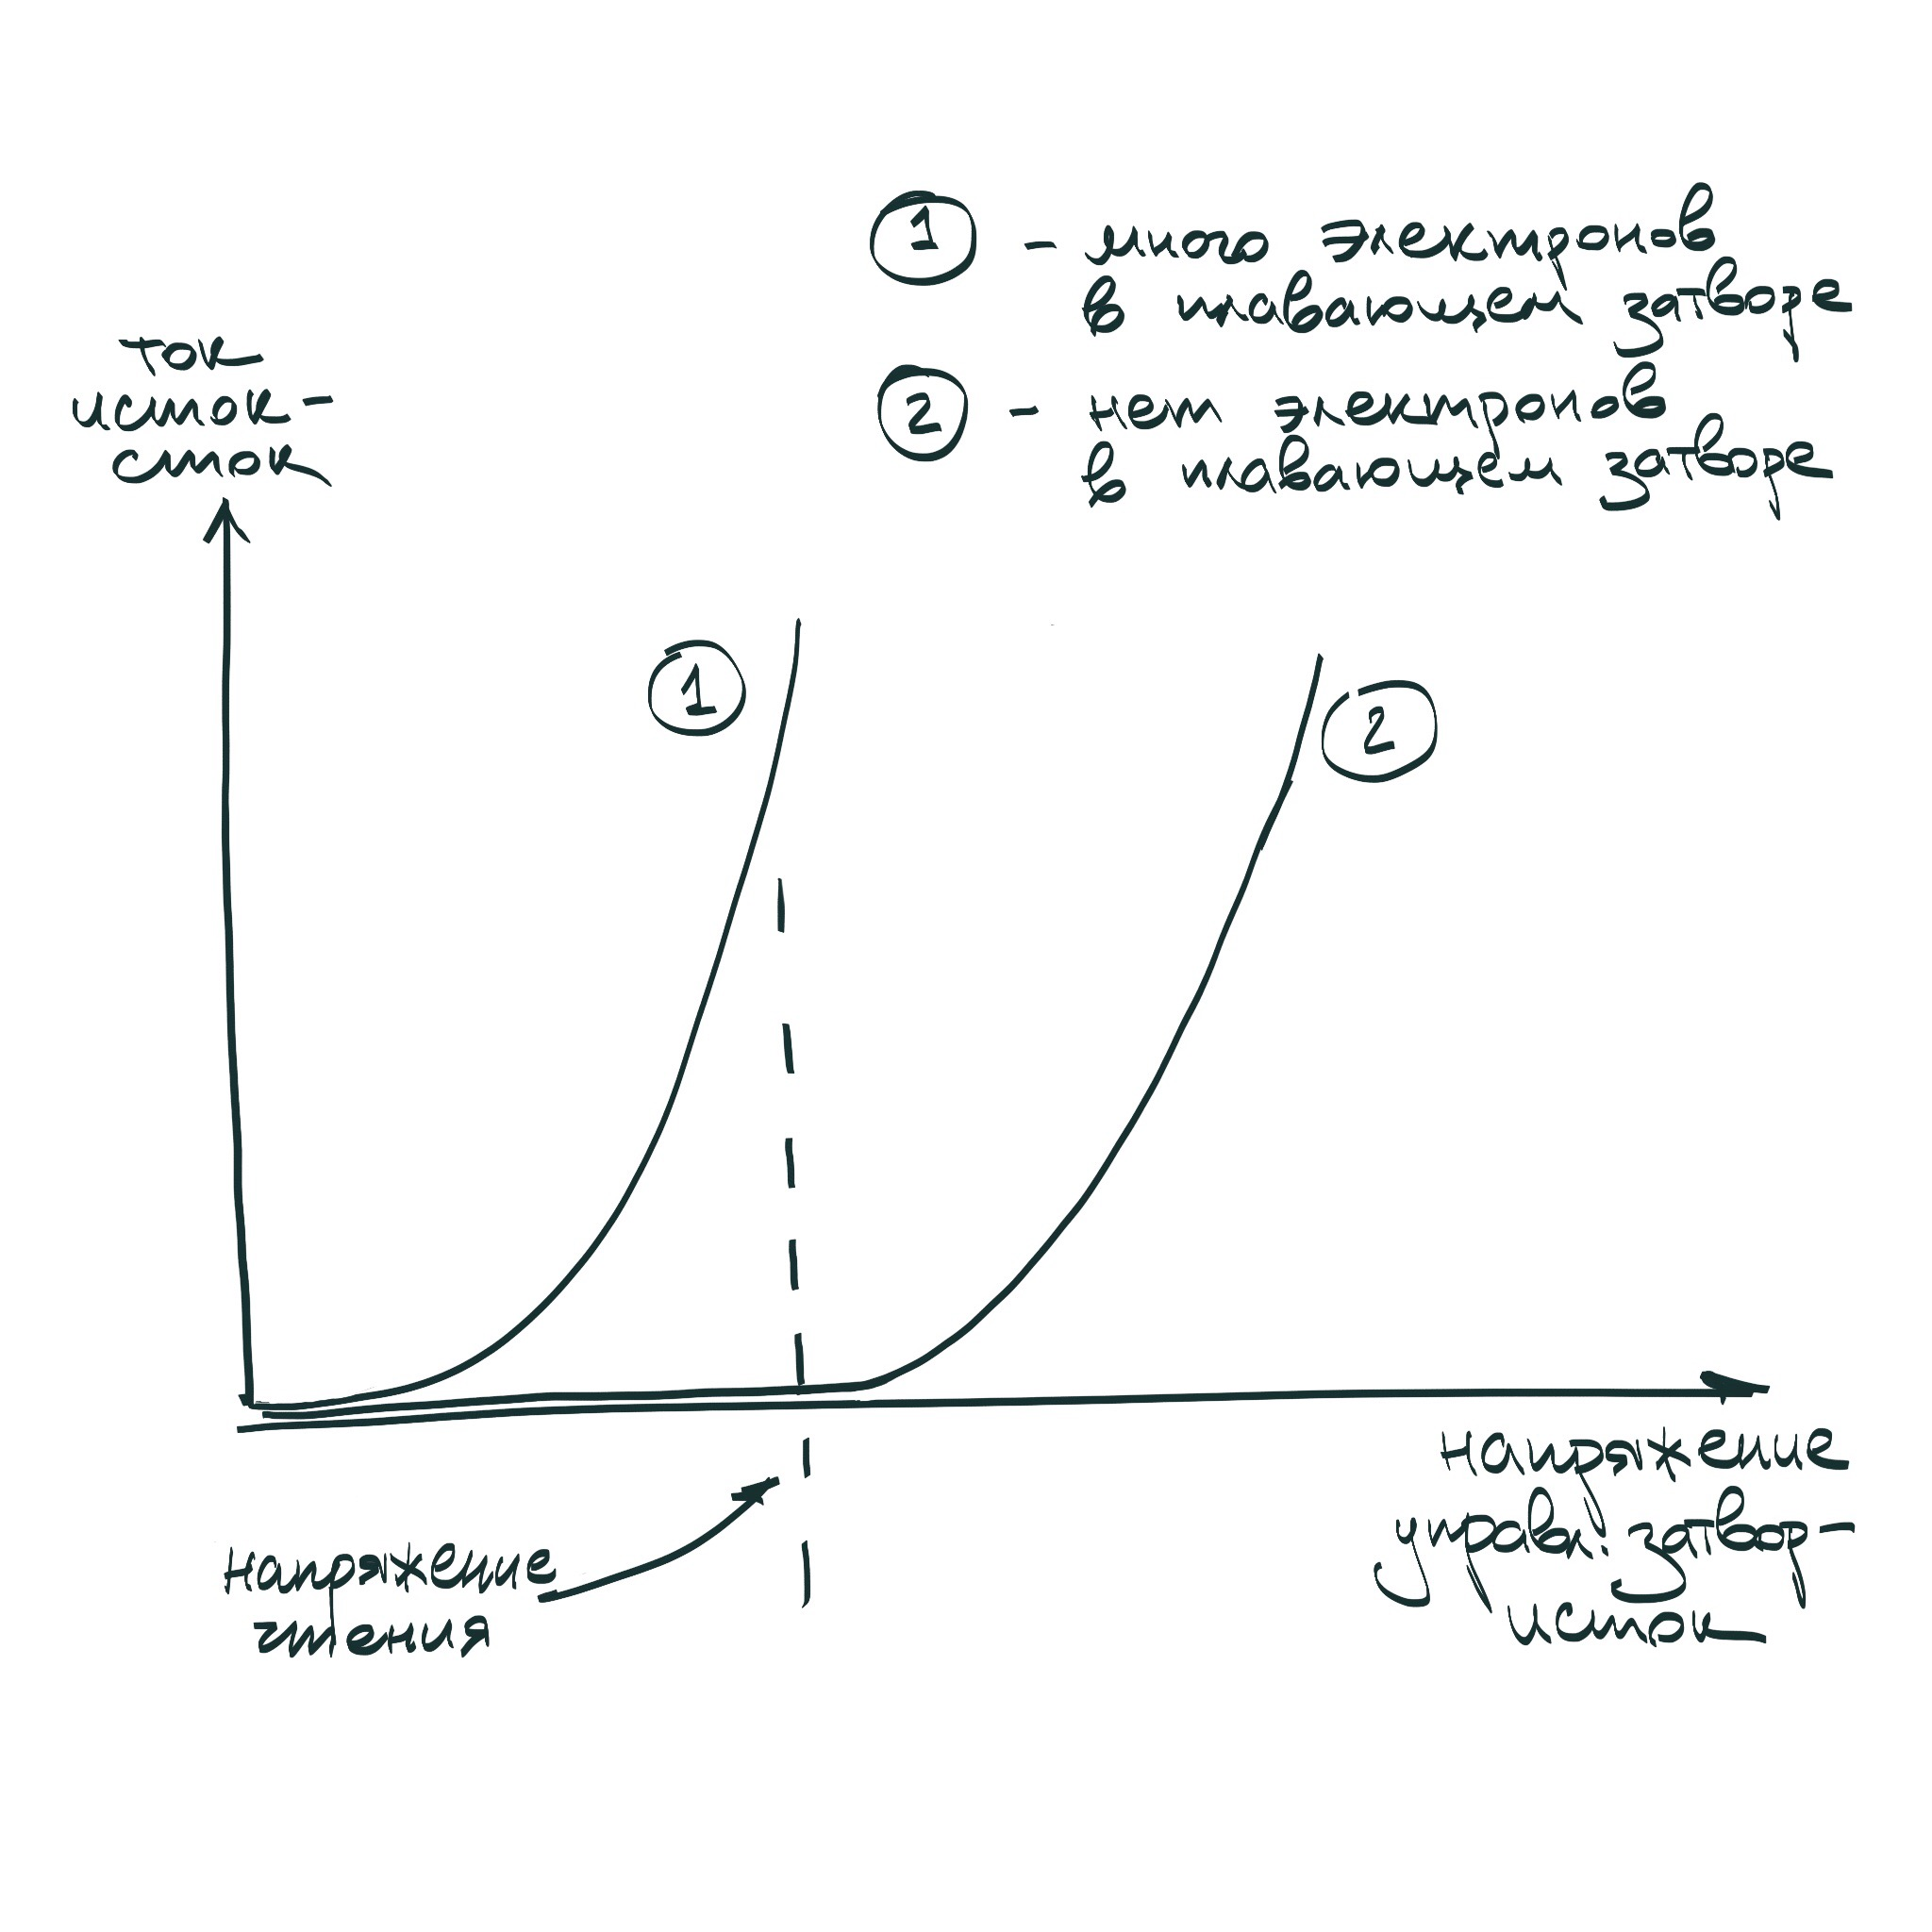
\includegraphics[width=0.8\textwidth]{./images/lab_6/floating_gate_read}
\caption{Чтение значение из транзистора с плавающим затвором}
\label{fig:floating_gate_read}
\end{figure}

\par{Осталось понять как можно \quotes{заставить} электроны попадать в плавающий затвор, ведь он изолирован диэлектриком. Не вдаваясь в подробности скажем, что если подать достаточно высокое напряжение \quotes{управляющий затвор---сток}, то у электронов хватит энергии, чтобы \quotes{перескочить} диэлектрик и попасть в плавающий затвор. А если изменить полярность этого напряжения, то можно \quotes{выгнать} электроны наружу (см. Рис.\ref{fig:floating_gate_change}).}

\begin{figure}[H]
\centering
% \def\svgwidth{\columnwidth}
% \includesvg{floating_gate_read}
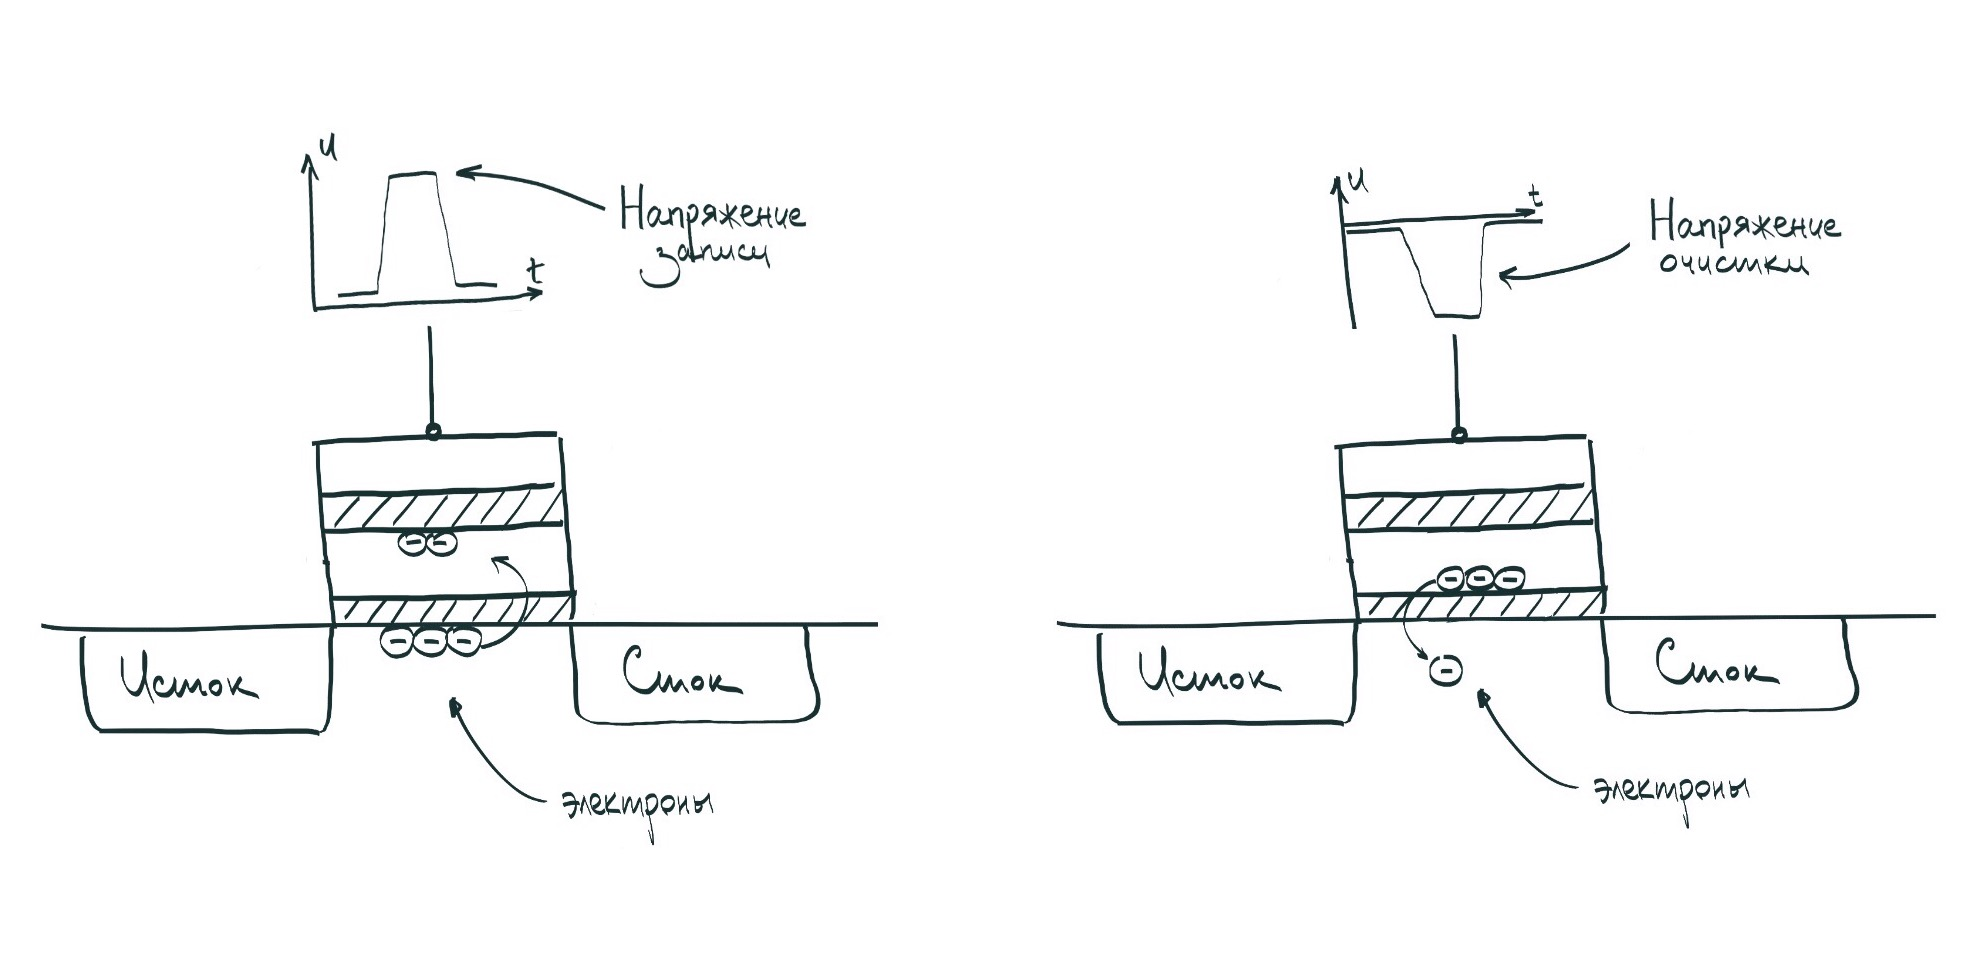
\includegraphics[width=0.8\textwidth]{./images/lab_6/floating_gate_change}
\caption{Изменение состояния плавающего затвора}
\label{fig:floating_gate_change}
\end{figure}

\par{Самое важное в этой идее то, что если электроны попали в плавающий затвор они не могут самостоятельно покинуть его через диэлектрик и будут оставаться там в течении многих лет. Таким образом и достигается сохранение записанной информации при отсутствии питания.}

\par{Теперь мы знаем, что для того чтобы записать или считать информацию из \eng{FLASH}-памяти надо использовать большую разность потенциалов. Но на самом деле транзистор устроен таким образом, что энергия, необходимая чтобы \quotes{загнать} электроны в плавающий затвор меньше энергии, необходимой, чтобы их \quotes{выгнать}. Это делается чтобы при чтении значения электроны не покидали плавающий затвор.}

\par{При такой организации становится сложно обеспечить очистку каждого транзистора в отдельности, поэтому обычно стирается целая группа ячеек.}

\section{Особенности \eng{FLASH}-памяти}

\par{Из-за особенностей транзистора с плавающим затвором, которые мы рассмотрели можно выделить следующие характерные черты \eng{FLASH}-памяти:
\begin{itemize}
  \item Запись значения возможна только из логической \quotes{1} в логический \quotes{0};
  \item Удаление информации возможно только из группы ячеек одновременно (сектора);
  \item Удаление и запись информации приводят к деградации ячеек памяти;
  \item Чтение также приводит к деградации ячеек памяти, но в меньшей степени.
\end{itemize}}

\section{Структура \eng{FLASH}-памяти}

\par{На Рисунке \ref{fig:flash_block_diagram} изображена общая структура \eng{FLASH}-памяти. Как видно она практически не отличается от \eng{RAM}-памяти: из ячеек строится матрица, контролируемая управляющим блоком. А сам управляющий блок обеспечивает коммуникацию с внешними устройствами, дешифрацию адреса и управление записью и чтением массива элементов памяти. Подключение \eng{FLASH}-памяти и управление ей со стороны цифрового устройства полностью зависит от того, как реализован блок управления --- доступ к содержимому \eng{FLASH}-памяти может быть синхронный или асинхронный, по последовательной или параллельной шине, с разделением шин адреса и данных или без него.}

\begin{figure}[H]
\centering
% \def\svgwidth{\columnwidth}
% \includesvg{flash_read_wave}
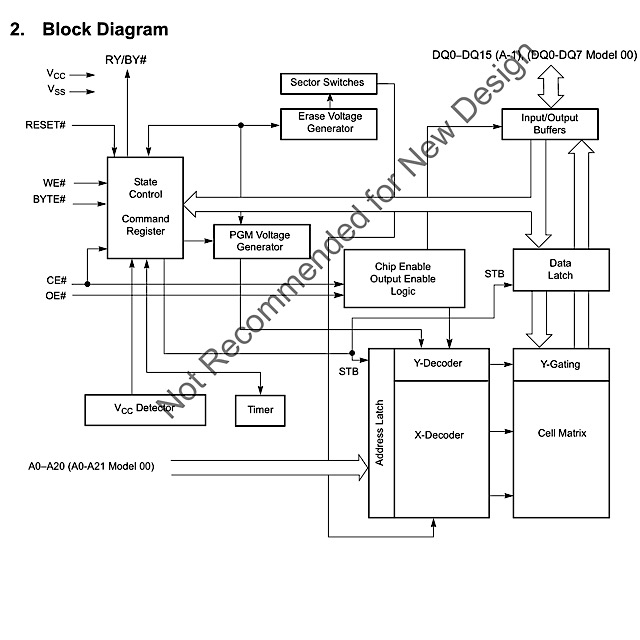
\includegraphics[width=0.8\textwidth]{./images/lab_6/flash_block_diagram}
\caption{Структура \eng{flash}-памяти \eng{S29AL032D}}
\label{fig:flash_block_diagram}
\end{figure}

\section{Микросхема \eng{FLASH}-памяти \eng{S29AL032D}}

\par{Для практического знакомства с \eng{FLASH}-памятью мы спроектируем контроллер микросхемы \eng{S29AL032D}. Именно эта микросхема установлена на отладочной плате Altera DE1.}
\par{Основным источником информации о любой микросхеме служат технические условия (англ. \eng{datasheet}). В этом документе содержатся все необходимые сведения для использования микросхемы: электрические параметры, размеры и тип корпуса, информация о выводах, и многие другие сведения. В том числе \eng{datasheet} содержит данные о протоколах информационного обмена.}
\par{В нашем случае микросхема уже подключена, поэтому из всего \eng{datasheet} нас, в первую очередь, интересует каким образом необходимо взаимодействовать с этой микросхемой, чтобы записать или считать данные.}
\par{Для разработки контроллера следует ознакомиться со следующими разделами документа:
\begin{itemize}[noitemsep,label={}]
  \item 11. \eng{Commands Definitions};
  \item 12. \eng{Write Operation Status};
  \item 17. \eng{AC Characteristics}.
\end{itemize}}
\par{Далее будут приведены необходимые выдержки из документа, однако настоятельно рекомендуем ознакомиться с ним.}

\subsection{Проектирование контроллера \eng{S29AL032D}}
\par{Как мы уже знаем, контроллер предназначен для обмена информацией с внешними цифровыми устройствами. Он должен предоставлять удобный, простой интерфейс и обеспечивать все необходимые взаимодействия с устройством. В таком случае другие блоки могут использовать один и тот же контроллер.} 
\par{Чтобы начать разработку контроллера, нужно ответить важные вопросы: как должен работать наш контроллер и как он должен управляться?}
\par{Если мы хотим работать с памятью, то для нас наиболее важными являются операции записи и чтения данных.  Тогда наиболее удобным для нас был бы уже знакомый интерфейс, похожий на \eng{RAM}-память: данные для записи, данные для чтения, адрес и управляющие сигналы.}
\par{Теперь, когда мы определились с тем, как мы будем управлять контроллером, нам нужно понять как он должен взаимодействовать с самой микросхемой \eng{FLASH}-памяти. Для этого изучим информацию о самой микросхеме и  операциях записи и чтения, описанные в \eng{datasheet S29AL032D}.}

\subsection{Операция чтения}
\par{Важной особенностью микросхемы \eng{S29AL032D} является использование двунаправленной шины данных. Это сделано для минимизации разводки печатной платы при её использовании. В дальнейшем нам придется разработать механизм, позволяющий использовать одну шину и для операции чтения и для операции записи.}
\par{Чтение данных из микросхемы \eng{S29AL032D} не требует никакой дополнительной подготовки. Временная диаграмма чтения приведена в пункте 17.2 \eng{datasheet} и представлена на Рисунке\ref{fig:flash_read_op}.}
\par{Времена, указанные на диаграмме, приведены в Таблице \ref{table:flash_read_timings}.}

\begin{figure}[H]
\centering
% \def\svgwidth{\columnwidth}
% \includesvg{flash_read_op}
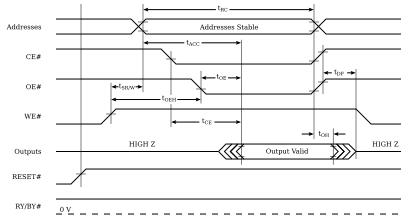
\includegraphics[width=0.8\textwidth]{./images/lab_6/flash_read_op}
\caption{Временная диаграмма чтения \eng{S29AL032D}}
\label{fig:flash_read_op}
\end{figure}

% \tabcolsep=0.11cm
\begin{table}[htbp]
  \centering
  \footnotesize
  \begin{tabular}{l|l|c|c}
    Обозн. & Описание & \eng{Min} & \eng{Max} \\
    \hline
    $t_{RC}$ & Продолжительность цикла чтения & 70 нс & --- \\
    $t_{ACC}$ & Задержка Адрес --- Данные & --- & 70 нс \\
    $t_{CE}$ & От активного \eng{CE} до формирования выхода & --- & 70 нс \\
    $t_{OE}$ & От активного \eng{OE} до формирования выхода & --- & 30 нс \\
    $t_{DF}$ & От снятия \eng{CE} до Z-состояния выхода & --- & 16 нс \\
    $t_{SR/W}$ & Задержка между операциями чтения и записи & 20 нс & ---\\
    $t_{OEH}$ & Время активного сигнала \eng{OE} & 10 нс & ---\\
    $t_{OH}$ & Время удержания данных & 0 нс & ---\\
  \end{tabular}
  \caption{Временные характеристики операции чтения \eng{S29AL032D} в режиме 70 нс.}
  \label{table:flash_read_timings}
\end{table}

\par{Чтобы выполнить операцию чтения, нам нужно повторить эту временную диаграмму и соблюсти все временные интервалы. Но как это сделать?}

\par{Каким образом можно выдержать указанные временные интервалы?}
\par{Мы уже знаем, что единственным источником информации о времени для цифрового устройства может являться только сигнал синхронизации, частота которого заранее известна.}
\par{Привяжем времена, упомянутые в Таблице \ref{table:flash_read_timings} к тактовому сигналу частоты 50 МГц, которым тактируется устройство. При этом учтём, что некоторые задержки могут быть равны нулю.}
\par{Полученная временная диаграмма показана на Рисунке \ref{fig:clocked_flash_read}}

\begin{figure}[H]
\centering
\begin{tikztimingtable}[%
    timing/dslope=0.1,
    timing/.style={x=5ex,y=2ex},
    x=5ex,
    timing/rowdist=3ex,
    timing/name/.style={font=\sffamily\scriptsize},
]
  CLK50        & 11{c} \\
  ADDRESS      & .5U 4D{Read\ Addr.} 2u \\
  \nsig{CE}    & .5H 4L 1H \\
  \nsig{OE}    & .5H 2H 2L 1H \\
  \nsig{WE}    & .5L 4H L \\
  DATA         & .5Z 3.5Z 0.2Z 0.1U 0.3D 0.9U \\
\extracode
\begin{pgfonlayer}{background}
\begin{scope}[semitransparent ,semithick]
\vertlines[darkgray,dotted]{1.5, 2.5, 3.5}
\vertlines[red]{0.5,4.5}
\end{scope}
\end{pgfonlayer}
\end{tikztimingtable}
\caption{Временная диаграмма операции чтения \eng{S29AL032D}, привязанная к тактовому сигналу, частотой 50 МГц.}
\label{fig:clocked_flash_read}
\end{figure}

\subsection{Операция записи}
\par{Обычно запись во \eng{FLASH}-память --- более сложная операция, чем чтение. Многие производители используют для записи специальные последовательности команд, защищая таким образом память от случайной записи.}
\par{Согласно \eng{datasheet S29AL032D} (разделы 7 и 11) для того, чтобы осуществить запись нужного значения во \eng{FLASH}-память, необходимо выполнить следующую последовательность из 4-х операций записи:
\begin{itemize}[noitemsep, label={}]
  \item Записать данные \eng{AA} по адресу \eng{AAA};
  \item Записать данные \eng{55} по адресу \eng{555};
  \item Записать данные \eng{A0} по адресу \eng{AAA};
  \item Записать нужные данные по нужному адресу.
\end{itemize}
}
\par{Временная диаграмма завершающей части одной операции записи приведена в пункте 17.4 \eng{datasheet} и представлена на Рисунке \ref{fig:flash_write_op}, а её временные характеристики приведены в Табл. \ref{table:flash_write_timings}.}

\begin{figure}[H]
\centering
% \def\svgwidth{\columnwidth}
% \includesvg{flash_write_op}
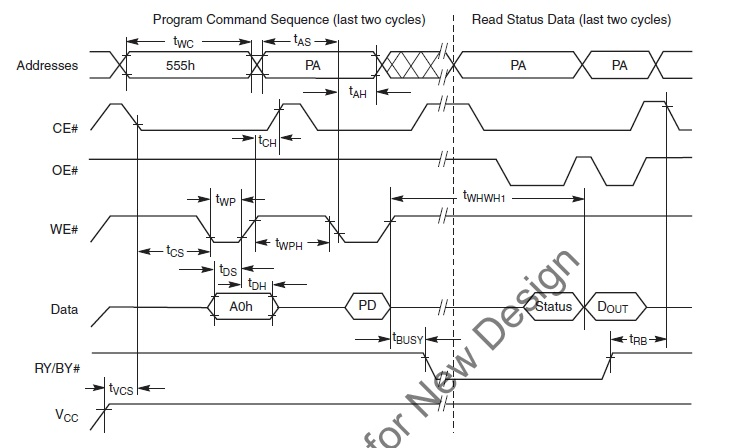
\includegraphics[width=0.8\textwidth]{./images/lab_6/flash_write_op}
\caption{Временная диаграмма фрагмента операции записи \eng{S29AL032D}}
\label{fig:flash_write_op}
\end{figure}

% \tabcolsep=0.11cm
\begin{table}[htbp]
  \centering
  \small
  \begin{tabular}{l|l|c|c}
    Обозн. & Описание & \eng{Min} & \eng{Max} \\
    \hline
    $t_{WC}$ & Продолжительность цикла записи & 70 нс & --- \\
    $t_{AS}$ & Время установки адреса & 0 нс & --- \\
    $t_{AH}$ & Время удерживания адреса & 45 & --- \\
    $t_{DS}$ & Время установки данных & 35 нс & --- \\
    $t_{DH}$ & Время удержания данных & 0 нс & --- \\
    $t_{CS}$ & Время установки сигнала CE & 0 нс & --- \\
    $t_{CH}$ & Время удержания сигнала CE & 0 нс & --- \\
    $t_{WP}$ & Ширина импульса записи & 35 нс & --- \\
    $t_{WPH}$ & Интервал между записью & 30 нс & --- \\ \cline{3-4}
    $t_{WHWH1}$ & Время программирования байта & \multicolumn{2}{c}{$\approx$ 9 мкс} \\ \cline{3-4}
    $t_{BUSY}$ & От активного \eng{CE} до установка выхода & 35 нс & 70 нс \\
    $t_{RB}$ & От активного \eng{OE} до установки выхода & --- & 30 нс \\
  \end{tabular}
  \caption{Временные характеристики операции записи \eng{S29AL032D} в режиме 70 нс.}
  \label{table:flash_write_timings}
\end{table}

\par{Аналогично операции чтения, привяжем форму и времена временной диаграммы записи к тактовому сигналу, частотой 50 МГц. Полученная диаграмма, представлена на Рис. \ref{fig:clocked_flash_write}}

\begin{figure}[H]
\centering
\begin{tikztimingtable}[%
    timing/dslope=0.1,
    timing/.style={x=5ex,y=2ex},
    x=5ex,
    timing/rowdist=3ex,
    timing/name/.style={font=\sffamily\scriptsize},
]
  CLK50        & 10{c} \\
  ADDRESS      & .5U 4D{Read\ Addr.} 2u \\
  \nsig{CE}    & .5H 4L 1H \\
  \nsig{OE}    & .5H 5H \\
  \nsig{WE}    & .5H 2L 2H L \\
  DATA         & .5U 4D{Write\ Data} 2u \\
\extracode
\begin{pgfonlayer}{background}
\begin{scope}[semitransparent ,semithick]
\vertlines[darkgray,dotted]{1.5, 2.5, 3.5}
\vertlines[red]{0.5,4.5}
\end{scope}
\end{pgfonlayer}
\end{tikztimingtable}
\caption{Временная диаграмма одного цикла операции записи \eng{S29AL032D}, привязанная к тактовому сигналу, частотой 50 МГц.}
\label{fig:clocked_flash_write}
\end{figure}

\par{Также согласно \eng{datasheet}, данные записываются не мгновенно. На то, чтобы провести операцию записи одного слова требуется порядка 11 мкс. Что приблизительно соответствует 550 тактам на частоте 50 МГц.}
\par{Также крайне важно, что при записи данных микросхема \eng{S29AL032D} может менять значение с \quotes{1} на \quotes{0}, но не наоборот!}
\par{Чтобы поменять значение с \quotes{0} на \quotes{1} требуется очистка целого фрагмента памяти, называемого сектором, либо полная очистка всей микросхемы!}
\par{Значит, для того, чтобы мы могли полноценно пользоваться микросхемой \eng{S29AL032D} нам потребуется реализовать в контроллере функции очистки.}

\subsection{Операция очистки}
\par{Для очистки выбранного сектора необходимо выполнить следующую последовательность операций:
\begin{itemize}[noitemsep, label={}]
  \item Записать данные \qeng{AA} по адресу \qeng{AAA};
  \item Записать данные \qeng{55} по адресу \qeng{555};
  \item Записать данные \qeng{80} по адресу \qeng{AAA};
  \item Записать данные \qeng{AA} по адресу \qeng{AAA};
  \item Записать данные \qeng{55} по адресу \qeng{555};
  \item Записать данные \qeng{30} по адресу сектора, который необходимо очистить.
\end{itemize}}
\par{Операция очистки сектора занимает существенное время, и пока она не закончится, невозможно произвести запись или чтение из \eng{FLASH}-памяти.}
\par{Операция полной очистки отличается только последним значением: для полной очистки данные \eng{30} записываются по адресу \eng{AAA}.}
\par{В \eng{datasheet} на \eng{S29AL032D} приведены следующие значения:
\begin{itemize}[noitemsep, label={}]
  \item Очистка сектора --- приблизительно 0.7 сек.
  \item Полная очистка микросхемы --- приблизительно 45 сек.
\end{itemize}}

\subsection{Статус операции}
\par{Для того, чтобы контролировать завершение операций записи и очистки, а также отслеживать ошибки, которые могут возникнуть в процессе их выполнения необходимо получить информацию о статусе операции. Способы получения этой информации и её содержание приведены в разделе 12 \eng{datasheet}. Далее мы отметим наиболее важные для нас моменты.}
\par{Так как на отладочном стенде \eng{Altera DE1}, которым мы пользуемся для проведения лабораторных работ, не разведён сигнал \eng{BUSY} микросхемы \eng{S29AL032D}, то единственным способом получения статуса является чтение информации из адреса, по которому производилась запись.}
\par{Если операция удачно завершена --- то будет получено значение, из указанного адреса. Для операции записи оно должно совпадать с тем, которое мы хотели записать, а для операции очистки должно содержать только единицы (8'hFF).}
\par{Если операция ещё не завершена, то биты [7:2] считанного значения будут содержать информацию о статусе операции. До окончания операции записи DQ[7] будет иметь значение противоположное записываемому (\quotes{0} при очистке) - это основной признак того, что полученные данные отражают статус операции. Информация о битах статусного пакета приведена в Таблице \ref{table:flash_status}}

\begin{table}[]
  \centering
  \small
  \begin{tabular}{l|c|c|c|c|c|c}

    Операция & DQ7 & DQ6 & DQ5 & DQ4 & DQ3 & DQ2 \\
    \toprule

    Запись & $\sim$DQ7 & \begin{tabular}{@{}c@{}}меняет \\ значение\end{tabular} & 0 & таймаут & --- & \begin{tabular}{@{}c@{}}не меняет \\ значение\end{tabular} \\
    \hline
    Очистка & 0 & \begin{tabular}{@{}c@{}}меняет \\ значение\end{tabular} &  0 & таймаут & 1 & \begin{tabular}{@{}c@{}} меняет \\ значение\end{tabular} \\
  \end{tabular}
  \caption{Значение разрядов статуса.}
  \label{table:flash_status}
\end{table}

\par{Обратите внимание, что при повторном чтении некоторые биты статусного пакета меняют своё значение на противоположное. Это сделано, чтобы убедиться, что операция чтения выполняется корректно и микросхема не \quotes{зависла}.}
\par{В информации о статусе операции есть важный признак: бит DQ[4] является признаком того, что время операции превысило максимально допустимое. Если этот бит принимает значение \quotes{1}, то во время операции произошла какая-то ошибка. В подавляющем большинстве случаев это происходит при попытке записи в ячейку памяти, уже содержавшую какое-то значение.}

\subsection{Проектирование контроллера Flash (продолжение)}
\par{Теперь, когда мы познакомились с операциями, которые предстоит выполнять контроллеру, мы можем продолжить его проектирование.}
\par{Контроллер должен обеспечивать чтение, запись и очистку микросхемы. Для этого он должен последовательно обмениваться данными и производить проверку статуса операций. Значит в качестве его основы следует применить конечный автомат. Ведь именно конечный автомат позволяет нам разделить режимы работы и реализовать алгоритмы работы в цифровых устройствах.}
\par{Начнём проектировать конечный автомат с начального состояния --- состояния бездействия. Будем постепенно наращивать его сложность и степень детализации, уточняя некоторые особенности.}

\par{Из состояния бездействия возможны три различных перехода: операция чтения, операция записи и операция очистки. После окончания этих операций автомат снова возвращается в состояние бездействия.}

\begin{figure}[H]
\centering
% \def\svgwidth{\columnwidth}
% \includesvg{flash_read_wave}
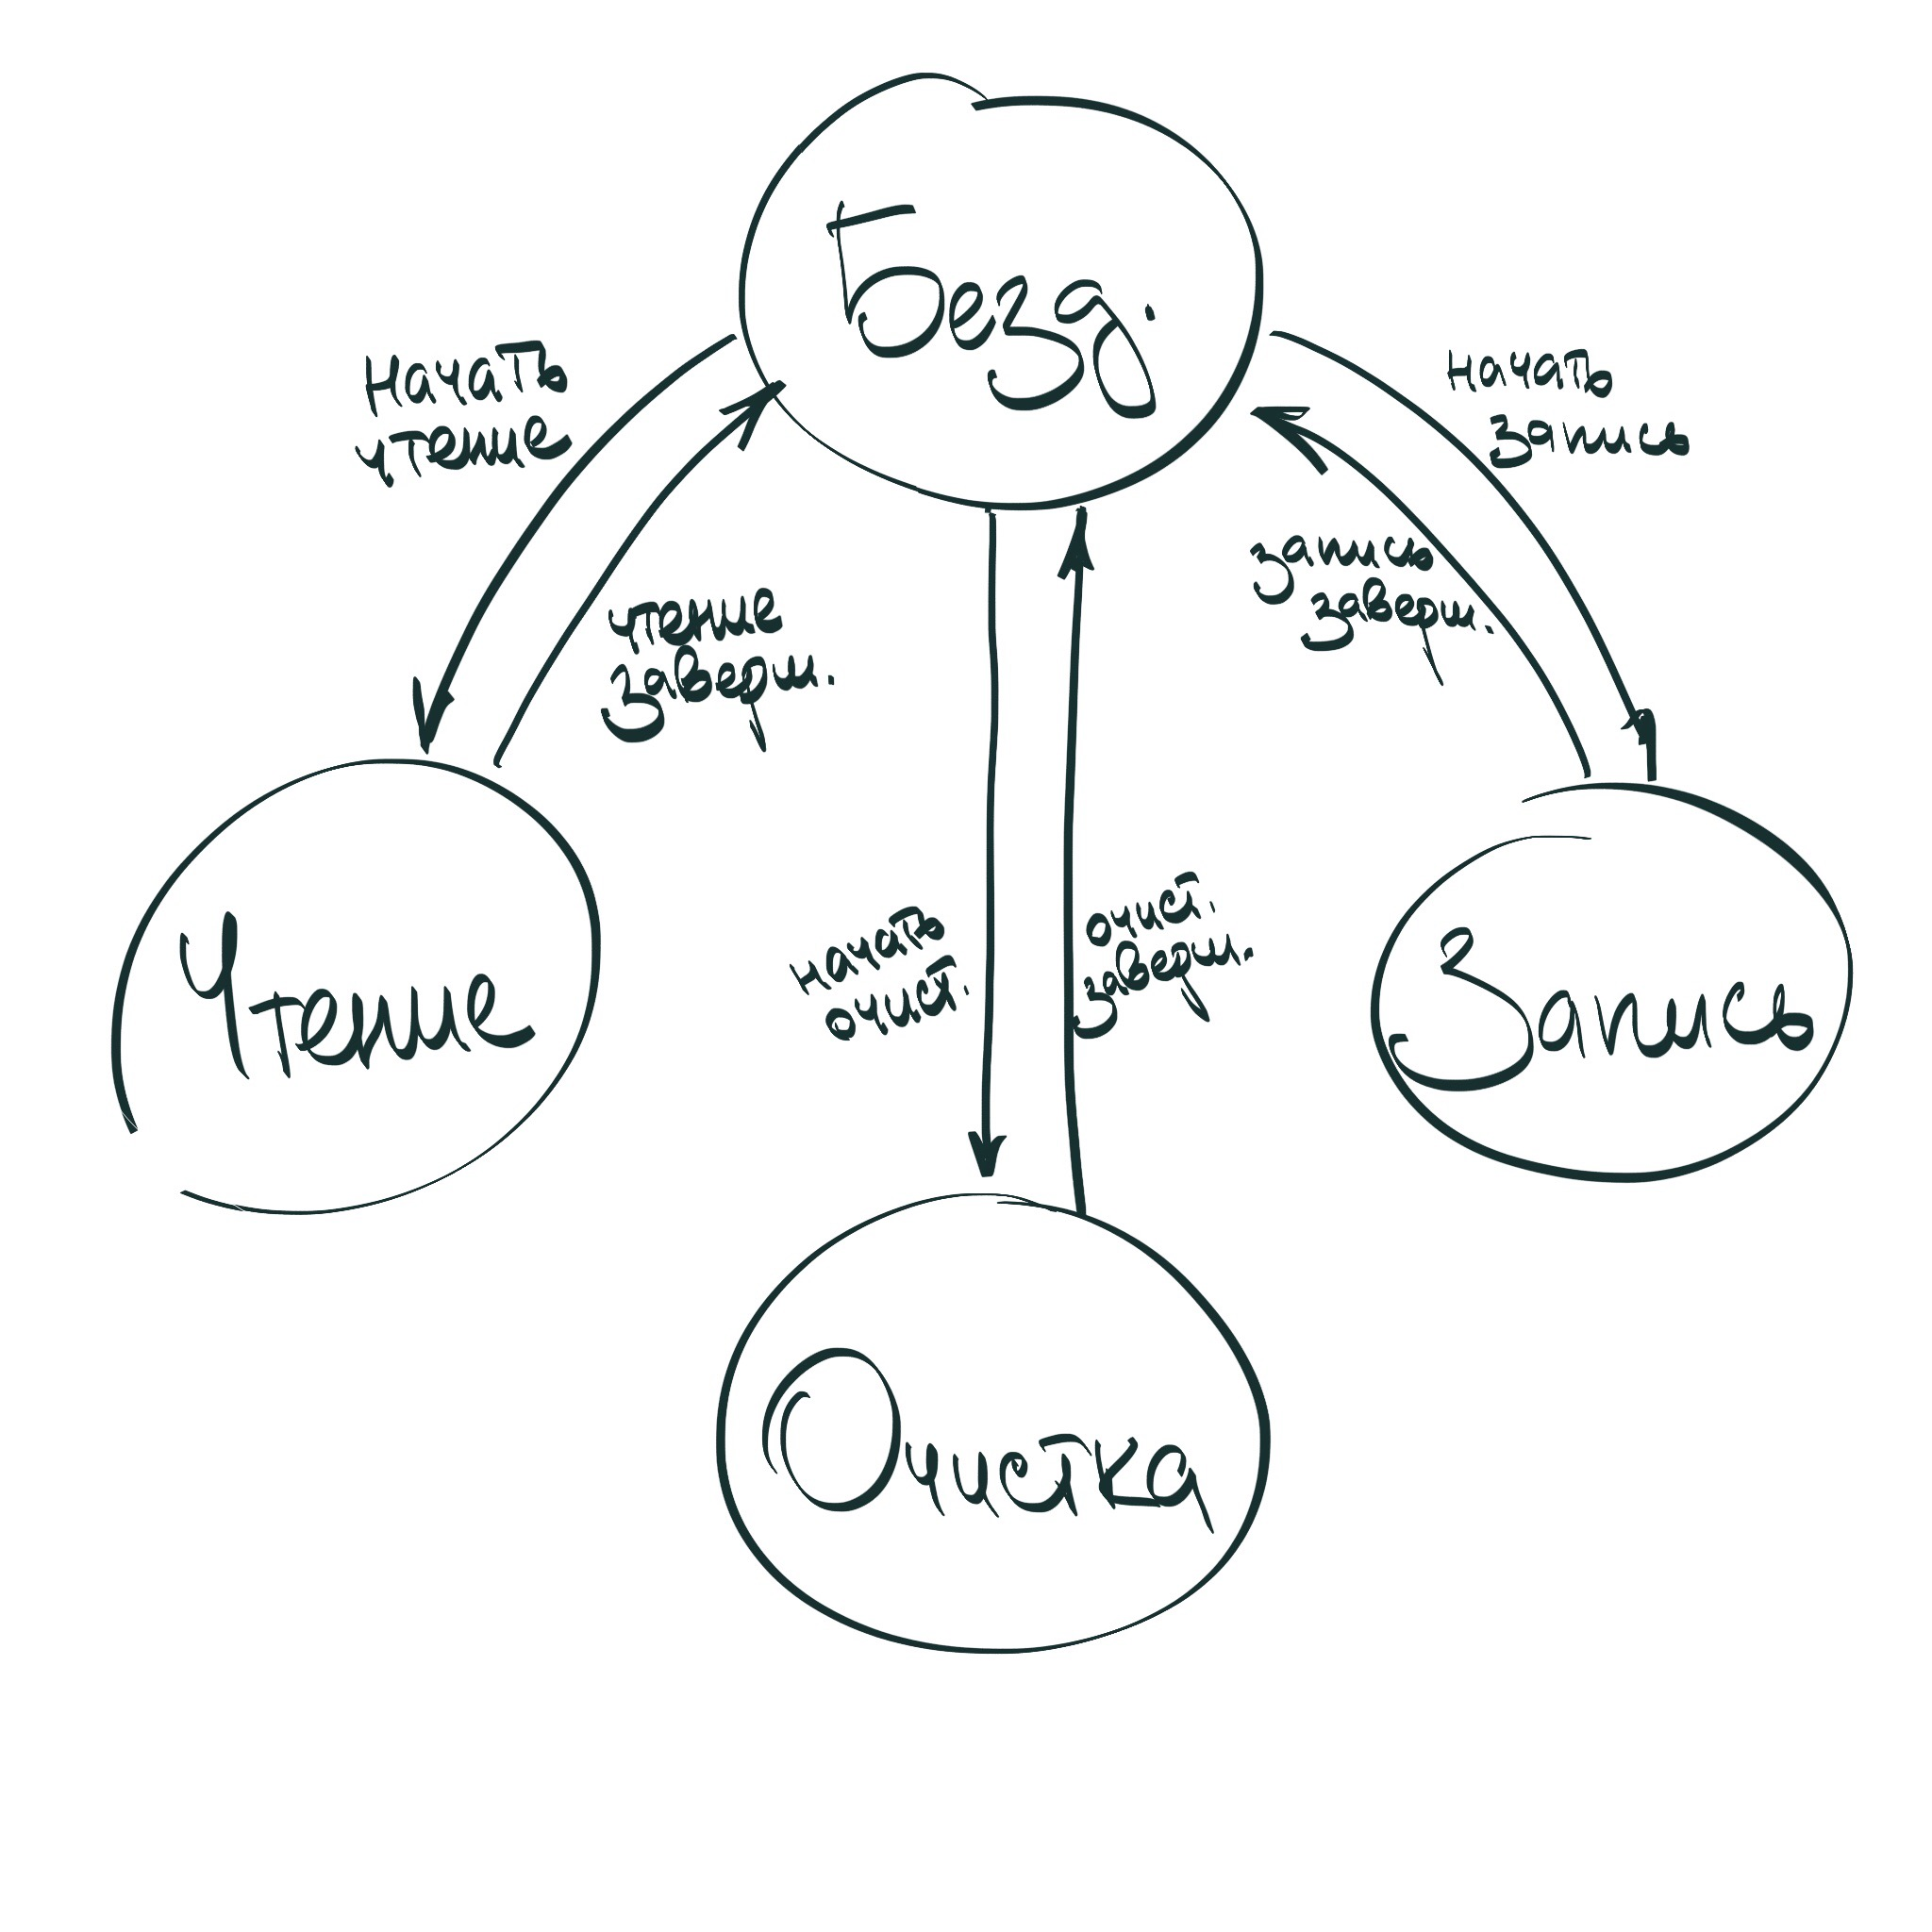
\includegraphics[width=0.8\textwidth]{./images/lab_6/fsm_simple}
\caption{Управляющий конечный автомат контроллера \eng{S29AL032D}}
\label{fig:fsm_somple}
\end{figure}

\par{Прежде всего, нас интересуют сложные операции \quotes{запись} и \quotes{очистка}. Выделим их основные этапы.}

\par{Как уже говорилось, чтобы записать данные во \eng{FLASH}-память требуется провести с ней четыре обмена. Но на этом нельзя заканчивать операцию, ведь необходимо дождаться окончания записи. Также надо учесть, что во время записи могут возникнуть ошибки.}
\par{Для контроля статуса операции нам нужно считать данные из адреса, по которому производится запись и проанализировать их.}
\par{Аналогичные рассуждения справедливы и для операции очистки. Отразим все эти замечания в состояниях конечного автомата (см. Рисунок \ref{fig:fsm_extended}).}

\begin{figure}[H]
\centering
% \def\svgwidth{\columnwidth}
% \includesvg{flash_read_wave}
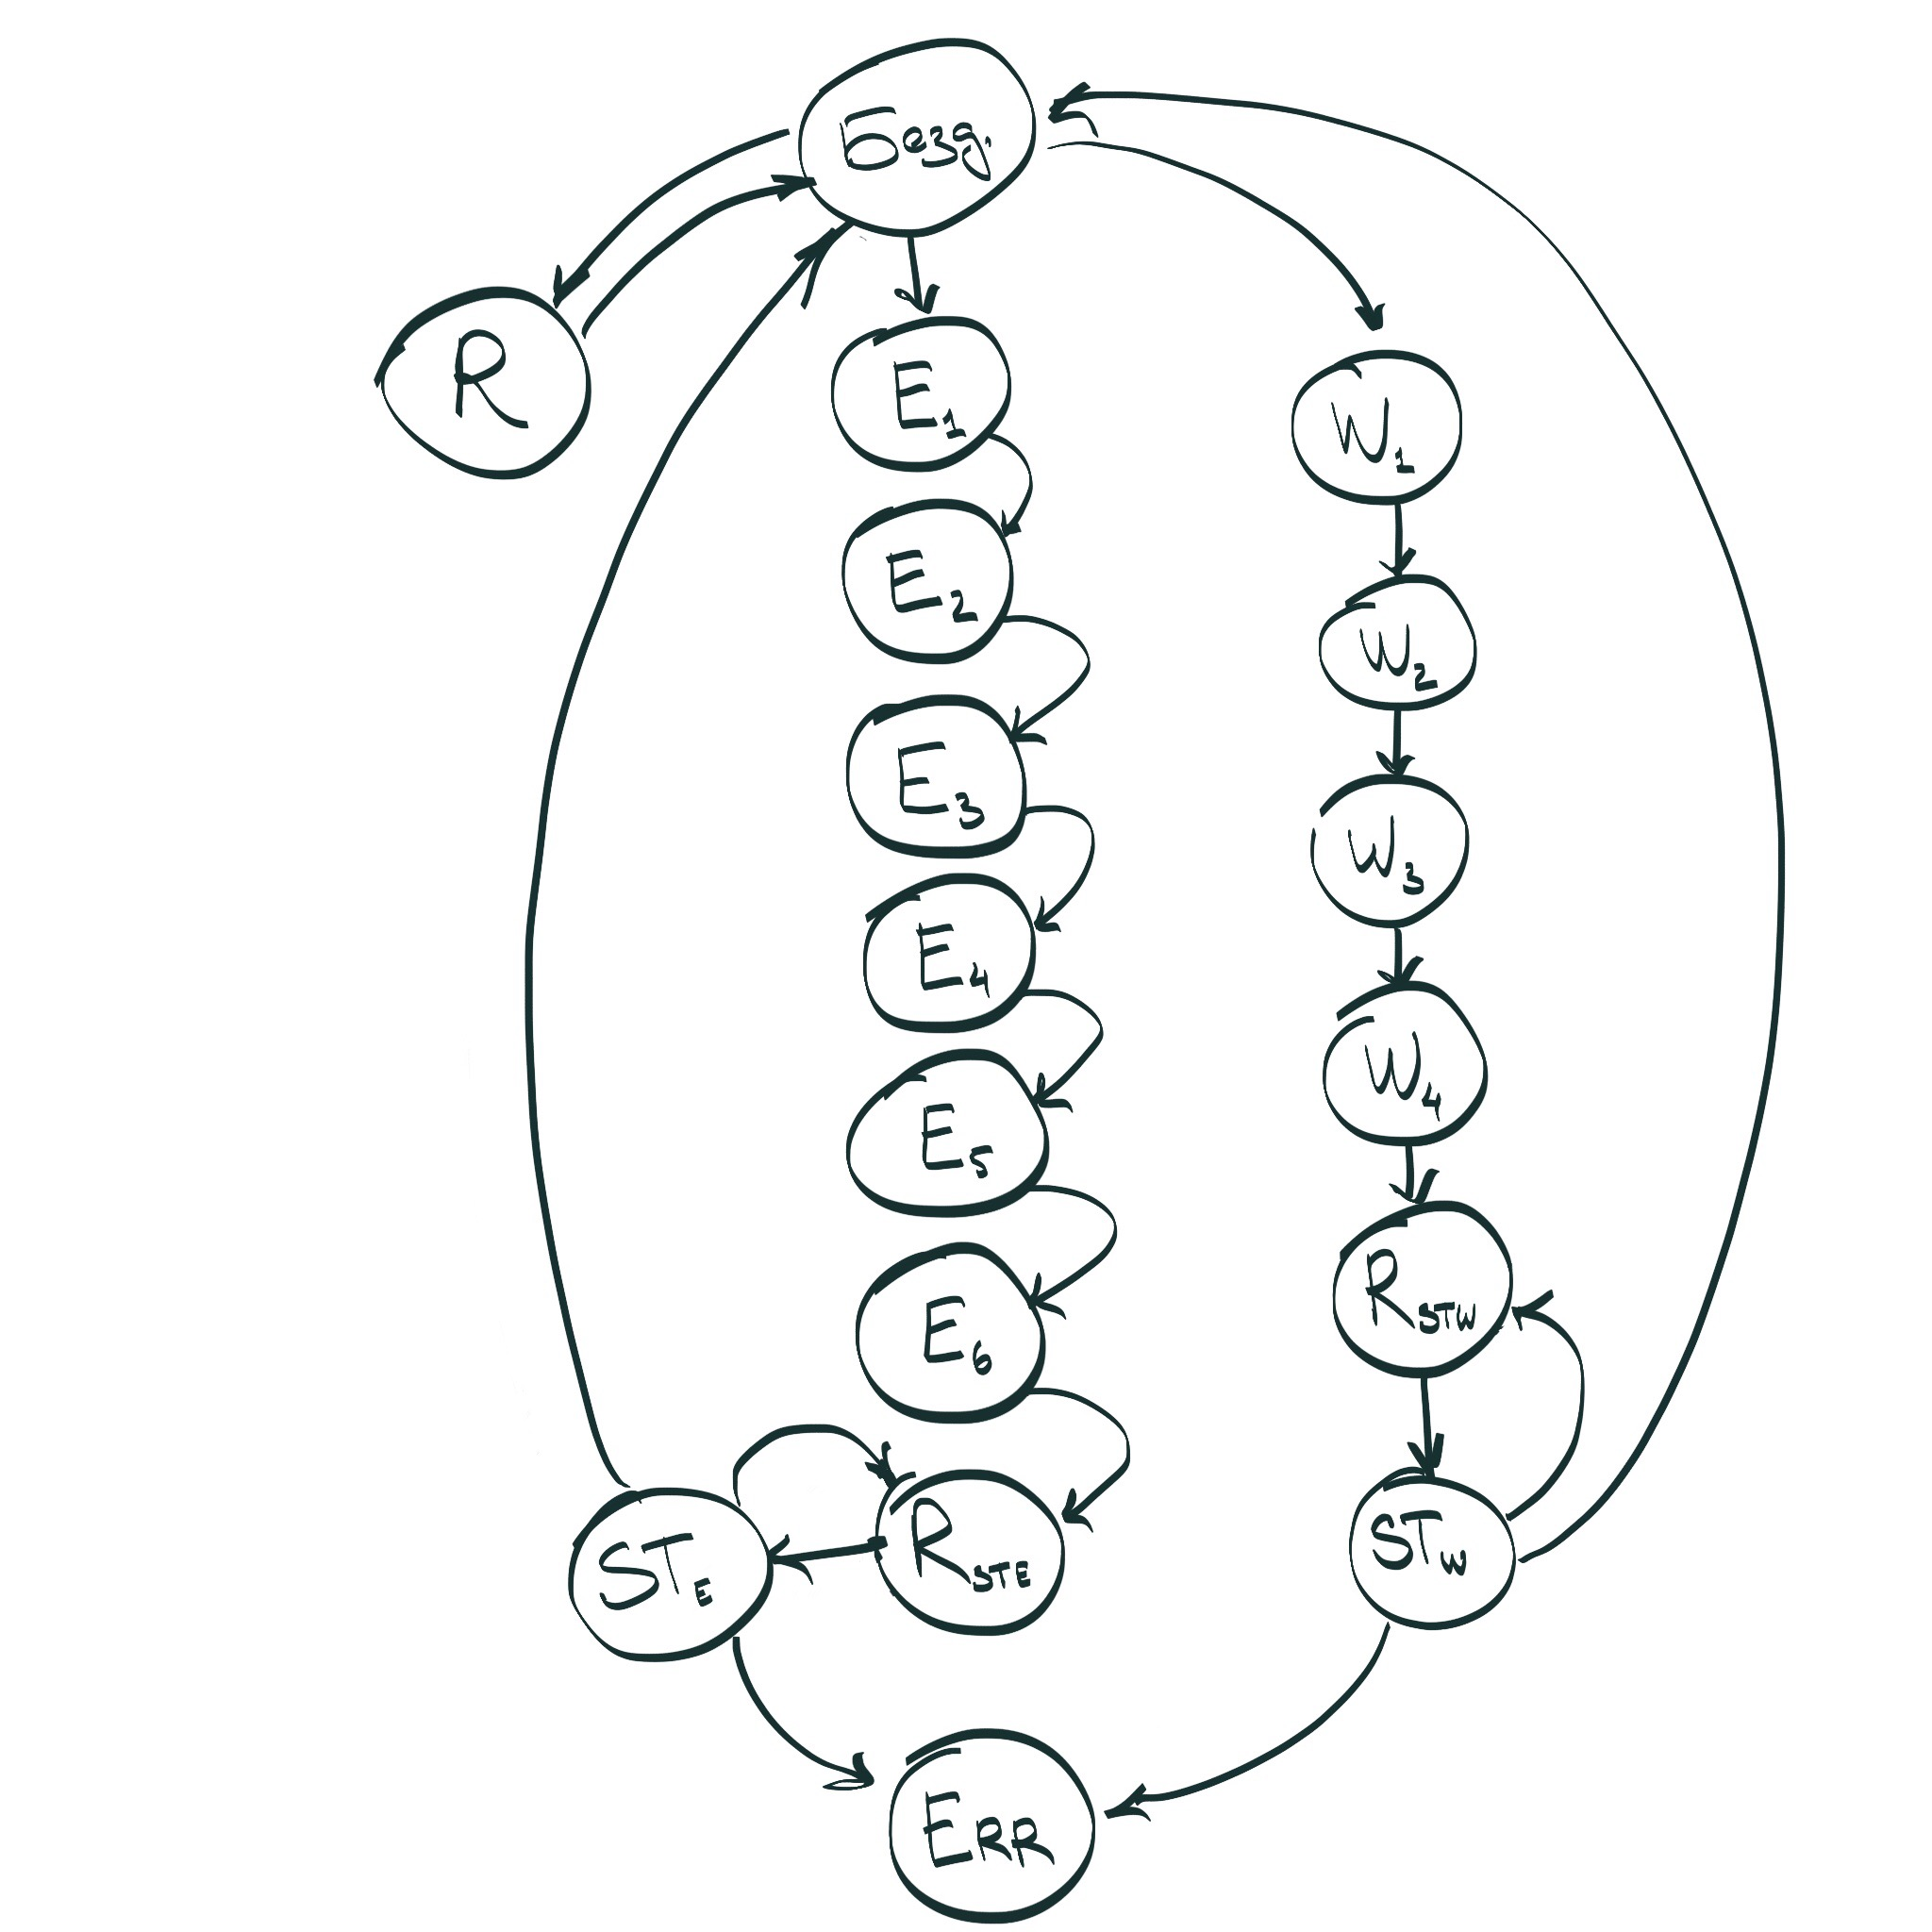
\includegraphics[width=0.8\textwidth]{./images/lab_6/fsm_extended}
\caption{Доработанный управляющий конечный автомат контроллера \eng{S29AL032D}}
\label{fig:fsm_extended}
\end{figure}

\par{Раньше мы не разделяли эти состояния $W_1 ... W_4, ST_w$ и всё вместе называли \quotes{запись}. Но, постепенно уточняя детали, мы разбили сложную операцию на более простые этапы.}
\par{Первое, что бросается в глаза в получившемся графе --- это многократное повторение операций записи в состояниях $W_1 ... W_4$ и $E_1 ... E_6$. Повторение операции чтения менее заметно: она происходит в сотояниях $R$ и $ST_W, ST_E$ (так как используется для проверки статуса).}
\par{Также можно постараться выделить анализ статуса $ST_W$ и $ST_E$ в состояние, общее для веток записи и очистки.}
\par{Тогда структура конечного автомата приобретает вид, показанный на Рисунке \ref{fig:fsm_common_status}}

\begin{figure}[H]
\centering
% \def\svgwidth{\columnwidth}
% \includesvg{flash_read_wave}
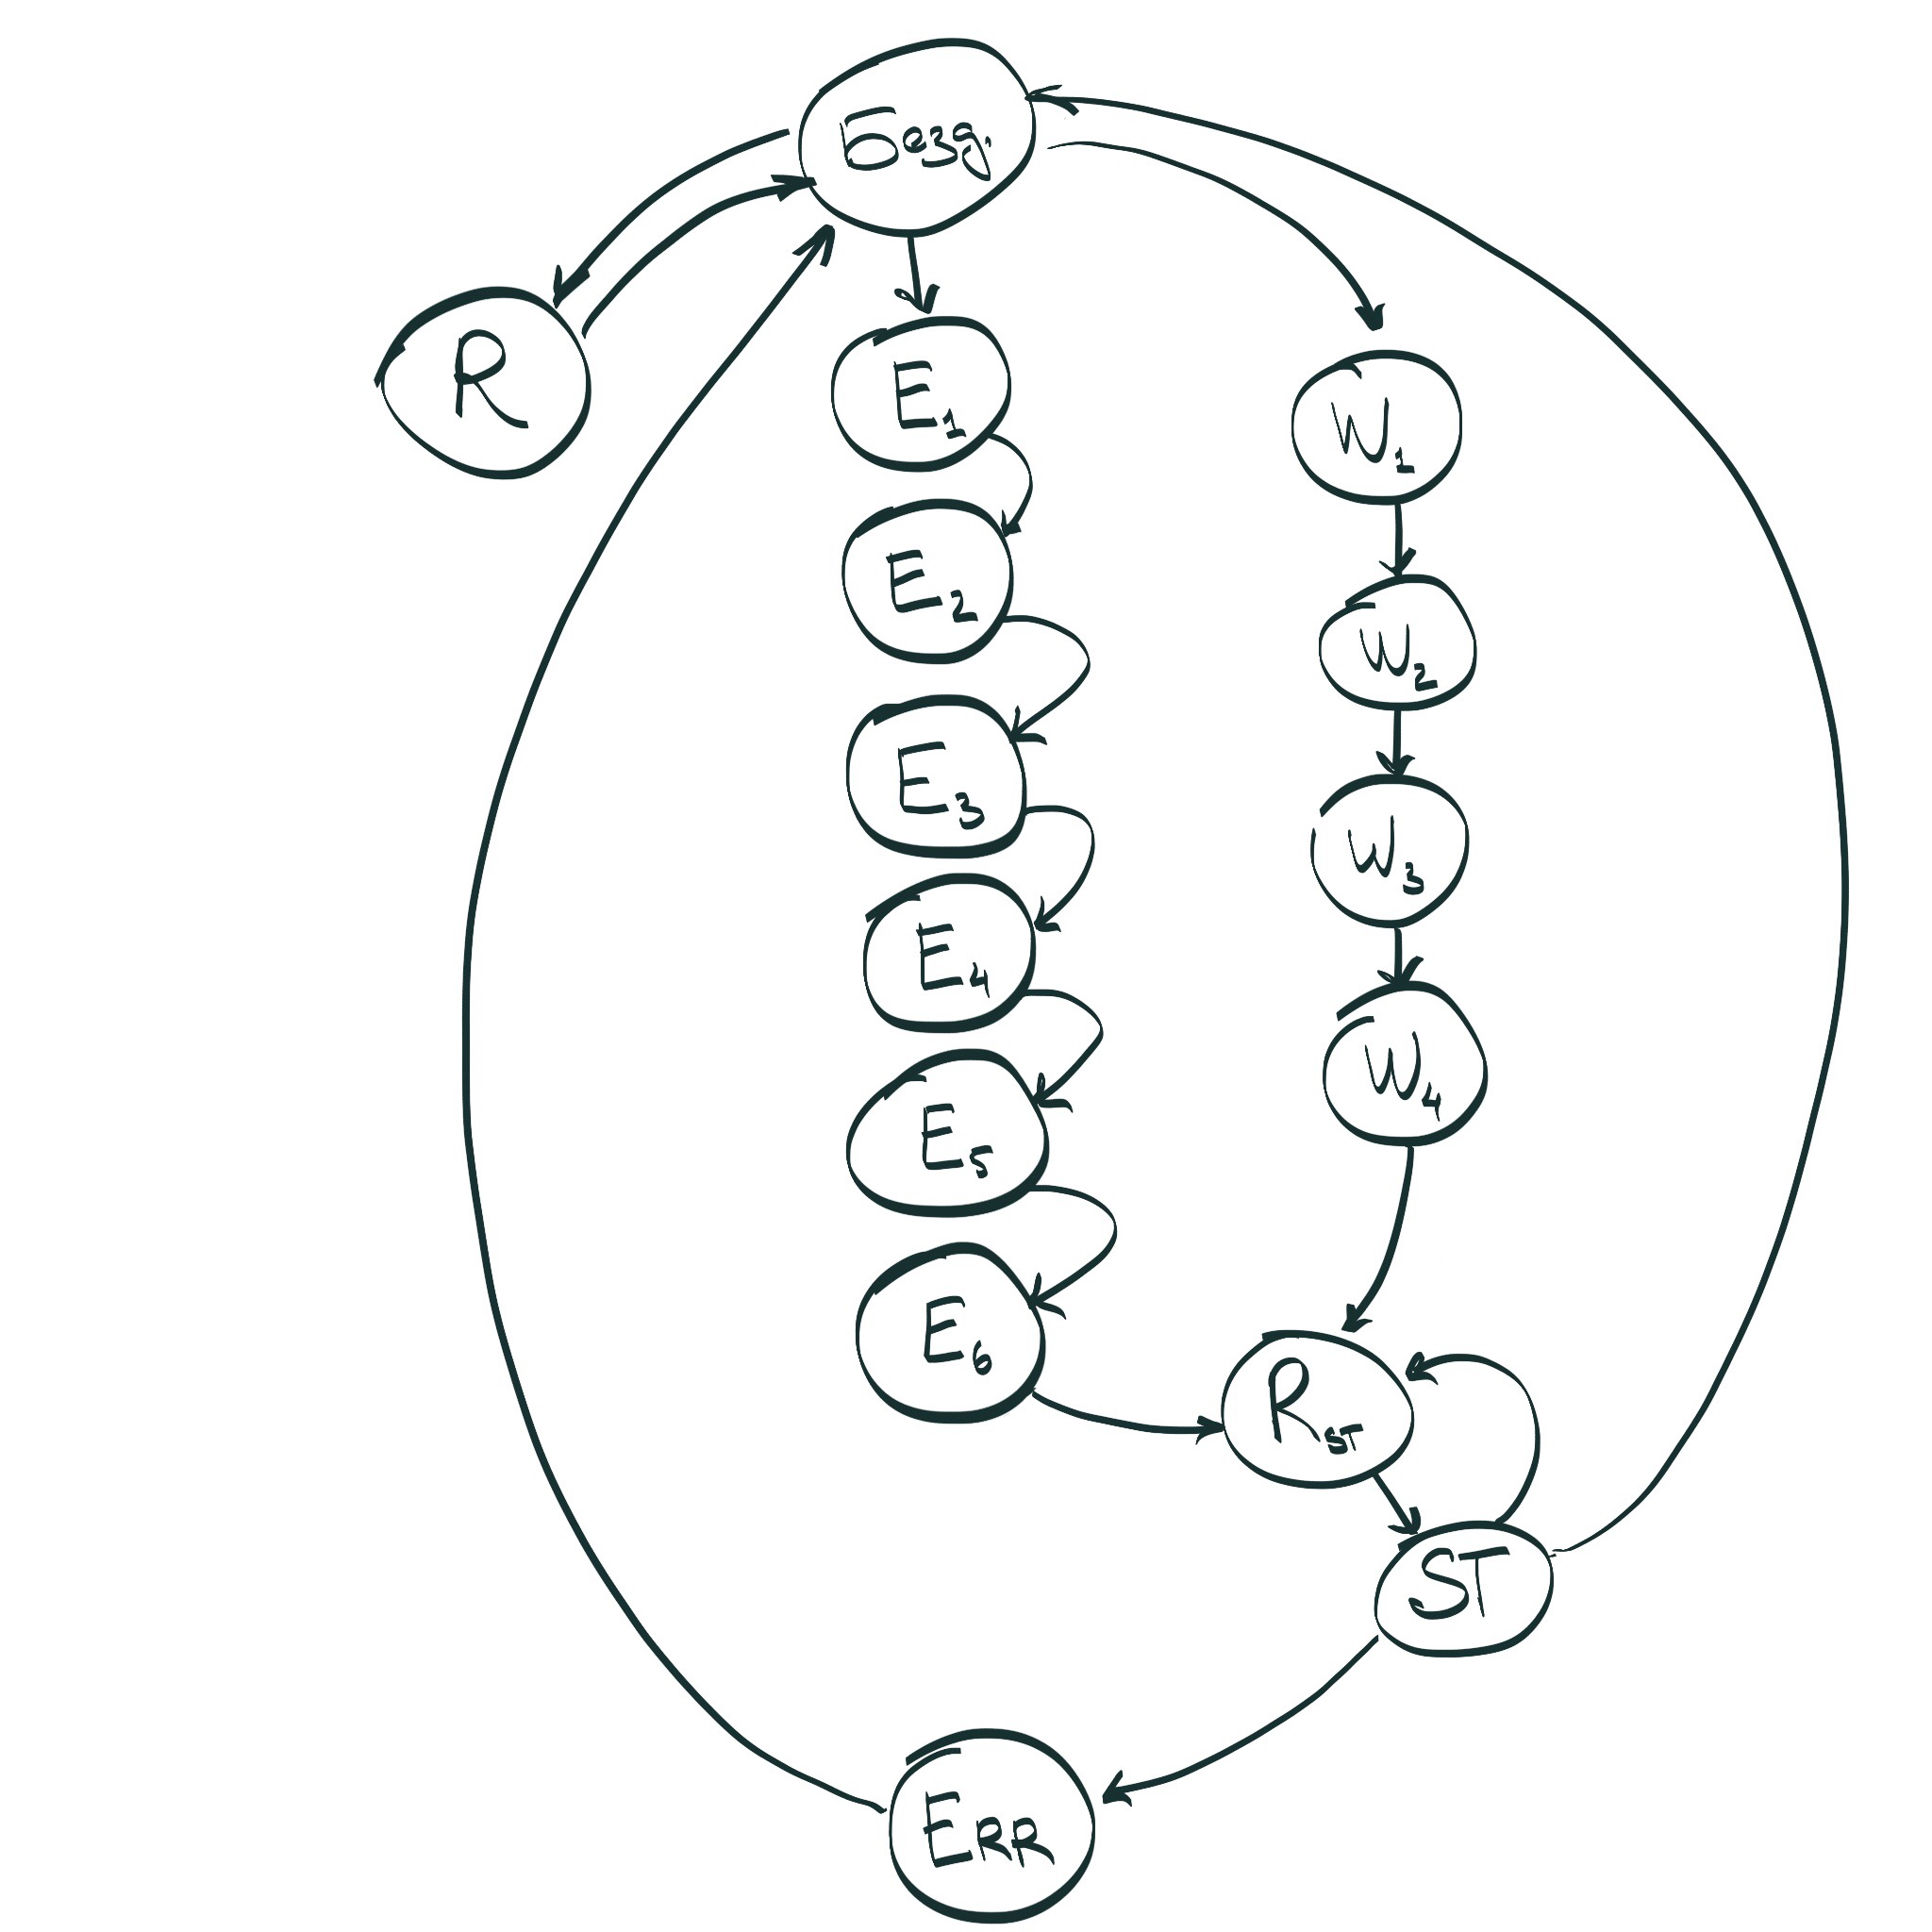
\includegraphics[width=0.8\textwidth]{./images/lab_6/fsm_common_status}
\caption{Конечный автомат контроллера \eng{S29AL032D} с общим состоянием проверки статуса}
\label{fig:fsm_common_status}
\end{figure}

\subsection{Реализация операций чтения и записи}
\par{Можем ли мы выделить операции чтения и записи и реализовать их отдельно, чтобы затем использовать их как показано на графе переходов?}
\par{Чтобы понять это, сначала ответим на вопрос как вообще возможно реализовать эти операции.}
\par{Для того, чтобы провести чтение, необходимо развернуть временную диаграмму, привязанную к тактовому сигналу, которую мы получили на Рисунке \ref{fig:clocked_flash_read}. Аналогичная временная диаграмма для записи была представлена на Рисунке \ref{fig:clocked_flash_write}.}
\par{Как мы уже обсуждали, схема которую можно использовать для разделения событий во времени --- это конечный автомат. Например, чтобы реализовать операцию чтения, разобьём временную диаграмму чтения на этапы, и поставим каждому этапу в соответствие уникальное состояние, как представлено на Рисунке \ref{fig:fsm_read_states}}

\begin{figure}[H]
\centering
\begin{tikztimingtable}[%
    timing/dslope=0.1,
    timing/.style={x=5ex,y=2ex},
    x=5ex,
    timing/rowdist=3ex,
    timing/name/.style={font=\sffamily\scriptsize},
]
  CLK50        & 11{c} \\
  ADDRESS      & .5U 4D{Read\ Addr.} 2u \\
  \nsig{CE}    & .5H 1H 3L 1H \\
  \nsig{OE}    & .5H 2H 2L 1H \\
  \nsig{WE}    & .5L 4H L \\
  DATA         & .5Z 3.5Z 0.2Z 0.1U 0.3D 0.9U \\
  \\
  STATE		   & .5U 1D{rr1} 1D{rr2} 1D{rr3} 1D{rr4} 1U\\
\extracode
\begin{pgfonlayer}{background}
\begin{scope}[semitransparent ,semithick]
\vertlines[darkgray,dotted]{1.5, 2.5, 3.5}
\vertlines[red]{0.5,4.5}
\end{scope}
\end{pgfonlayer}
\end{tikztimingtable}
\caption{Соответствие состояний этапам операции чтения \eng{S29AL032D}}
\label{fig:fsm_read_states}
\end{figure}

\par{Мы могли бы добавить эти состояния в конечный автомат, который мы уже начали проектировать, но тогда нам пришлось бы каждое из состояний $ST$, $RD$, $W_1 ... W_4$ и $E_1 ... E_6$, разбить на несколько состояний. Это привело бы к ненужному усложнению структуры конечного автомата и аппаратной избыточности.}
\par{Вместо этого мы можем сделать отдельные небольшие блоки, которые будут выполнять эти операции и, таким образом, разделить конченые автоматы автоматы.}
\par{Нам надо будет только предусмотреть, что для использования этих блоков надо предусмотреть механизмы запуска операции и сигнализации о окончании работы блока.}
\par{Сигналом запуска для таких блоков будет признак того, что основной автомат находится в состоянии \quotes{чтение} или \quotes{запись}, соответственно, а сигнал окончания работы будет вырабатываться в состоянии \quotes{завершено}.}
\par{Теперь, когда мы оформили все основные идеи и общую структуру контроллера, можно преступить к его реализации на \eng{Verilog HDL}.}

\subsection{Реализация контроллера микросхемы \eng{S29AL032D} на языке \eng{Verilog HDL}}
\subsubsection{Интерфейс}
\par{Как всегда, начнём проектировать с интерфейса будущего контроллера --- его входов и выходов. Так как контроллер будет обеспечивать доступ к памяти, мы хотели сделать его интерфейс похожим на интерфейс \eng{RAM}-памяти. Но нам придётся ввести дополнительные сигналы для того, чтобы реализовать операцию очистки и индикацию ошибок.}
\par{Нам будет достаточно одного входа для адреса, так как мы не можем одновременно производить чтение и запись во \eng{flash}-память. Но для данных, по аналогии с \eng{RAM}-памятью потребуются два отдельных входа --- для записи и для чтения.}

\noindent
  \lstinputlisting[caption={Описание интерфейса контроллера \eng{S29AL032D}}]{./code_examples/lab_6/flash_interface.v}

\subsubsection{Основной управляющий конечный автомат}
\par{Теперь опишем основной управляющий конечный автомат. Необходимо помнить, что данные, которые мы записываем во \eng{flash}-память нужно сохранить, чтобы они оставались неизменными все время выполнения операции. Поэтому сразу дополним описание регистром для хранения этих данных.}
\par{Сразу учтём, что эти же данные можно будет использовать для проверки статуса. Поэтому для операции очистки сектора, запишем в регистр 8'hFF.}
\noindent
  \lstinputlisting[caption={Описание управляющего конечного автомата контроллера \eng{S29AL032D}}]{./code_examples/lab_6/flash_main_fsm.v}

\pagebreak
\subsubsection{Конечный автомат чтения}
\par{Опишем автомат чтения и наладим связь между автоматами. Для этого опишем сигналы, которые понадобятся для управления каждым из этих автоматов.}

\noindent
  \lstinputlisting[caption={Описание конечного автомата чтения контроллера \eng{S29AL032D}}]{./code_examples/lab_6/flash_read_fsm.v}
  
\subsubsection{Проверка статуса операции}

\par{Мы заранее позаботились о том, чтобы проверка статуса не требовала от нас больших усилий: мы защелкиваем данные при начале операции записи и очистки. Теперь нам достаточно сравнить полученное значение с эталонным:}
\noindent
  \lstinputlisting[caption={Проверка статуса операции в контроллере \eng{S29AL032D}}]{./code_examples/lab_6/flash_status.v}

\subsubsection{Управление микросхемой \eng{S29AL032D}}
\par{Опишем поведение двунаправленной шины данных и сигналов управления для \eng{S29AL032D}. В состояниях чтения, шиной данный должна управлять микросхема, в состояниях записи --- контроллер:}

\noindent
  \lstinputlisting[caption={Управление микросхемой \eng{S29AL032D}}]{./code_examples/lab_6/flash_controls.v}

\pagebreak
\section{Задание лабораторной работы}

\begin{itemize}[noitemsep]
  \item Разработать конечный автомат записи;
  \item Разработать механизм передачи различных данных в состояниях $W_1, ..., W_4$ и $E_1, ..., E_6$;
  \item Выполнить полную интеграцию контроллера;
  \item Создать проект, для демонстрации возможностей контроллера, удовлетворяющий требованиям, представленным ниже.
\end{itemize}
\subsection{Требования к демонстрационному проекту}
\subsubsection{Режимы работы}
\par{С помощью $SW[1],SW[2]$ задается режим --- запись, чтение или очистка.}

\subsubsection{Сброс}
\par{Сброс устройства происходит по нажатию $BNT[0]$}
\subsubsection{Режим записи}
\par{В режиме записи с помощью кнопок $BTN[3], BTN[2]$ задается адрес записи, затем ввод подтверждается нажатием $BTN[1]$. Здесь и далее --- во время ввода, вводимое значение отображается на семисегментных индикаторах.}
\par{После подтверждения ввода адреса записи, с помощью кнопок $BTN[3], BTN[2]$ вводится записываемое значение и подтверждается нажатием $BTN[1]$.}
\par{После подтверждения ввода значения происходит запись в микросхему \eng{S29AL032D}. В случае успешной записи подсвечивается $LEDG[0]$ и демо-проект возвращается к вводу адреса записи, а в случае ошибки подсвечивается $LEDR[0]$.}

\pagebreak
\subsubsection{Режим чтения}
\par{В режиме чтения с помощью кнопок $BTN[3], BTN[2]$ задается адрес чтения, затем ввод подтверждается нажатием $BTN[1]$.}

\par{После подтверждения ввода адреса чтения, происходит чтение значения из микросхемы \eng{S29AL032D}. Считанное значение выводится на семисегментные индикаторы. После нажатия $BTN[1]$, устройство переходит в выбранный режим.}

\subsubsection{Режим очистки}
\par{В режиме очистки, с помощью кнопок $BTN[3], BTN[2]$ задается номер очищаемого сектора. Послед подтверждения ввода с помощью кнопки $BTN[1]$, производится выбранная операция.}
\par{После окончания операции в случае успешной очистки подсвечивается $LEDG[0]$, а в случае ошибки $LEDR[0]$.}



